%2.4 In addition, to assess the impacts of the reform the authors look at the effects on the perceptions of police performance by comparing perceptions between early and late adopters (Figure 4). To interpret this exercise, it would first be necessary that the authors provide evidence that adoption timing was not driven by differences in other pre-policy changes in local outcomes. Even if not all survey questions are available in every year, a regression of outcomes on the number of years of exposure to the policy could provide an alternative way to address this.

This is an excellent point, thank you very much. The reviewer noted that, to interpret this exercise, it would be necessary to show that adoption timing was not driven by differences in other pre-policy changes. Following reviewer's suggestion, we regress perceived police performance outcomes on the year of adoption of \emph{Plan Cuadrante}, restricting the sample to municipalities that had not yet adopted the program as of 2005, the year for which information on perceived police performance is available. The results, reported in panel (a) of Figure \ref{fig:balance_doseresponse}, show that perceived police performance before \emph{Plan Cuadrante} did not predict the timing of adoption.


Following your suggestion, as an additional exercise, we also reestimate the comparison reported in panel (a) of Figure 4, measuring years of exposure to \emph{Plan Cuadrante} in 2005 rather than simply whether the municipality had adopted the program. The results, reported in panel (b) of Figure \ref{fig:balance_doseresponse}, show the expected correlations, consistent with an increasing effect of \emph{Plan Cuadrante} on perceived police performance.

We have included the following footnote in Section 4.4 of the manuscript to reference these results:

\begin{adjustwidth}{2em}{0em}
Information on police performance is only available in ENUSC round 2005. Using this round, we compare perceived police performance in municipalities that adopted \emph{Plan Cuadrante} in 2005 or earlier and in municipalities adopting after 2005. Figure \ref{fig:balance_doseresponse} in Online Appendix \ref{sec:appendixB} shows that the number of years of exposure to \emph{Plan Cuadrante} is positively correlated with perceived police performance. While these exercises on perceived police performance should be interpreted with caution, we show in the same appendix that the timing of future adoption is not correlated with perceived police performance in 2005 for municipalities that had not yet adopted the program by 2005.
\end{adjustwidth}

And we added the following subsection, ``Adoption Timing and Perceived Police Performance,'' to Online Appendix B reporting this exercise in detail:

\begin{adjustwidth}{2em}{0em}
Information on perceived police performance is only available in the 2005 round of ENUSC, so the comparison in Figure \ref{fig:figure05} relies on a single cross-section, comparing municipalities that had already adopted \emph{Plan Cuadrante} by 2005 (early adopters) with those that had not yet done so (late adopters). We consider seven measures of perceived police performance: the share of respondents who perceive police performance as good, and who perceive the police to be efficient, helpful, well informed, corrupt, failing to control crime, and failing to do their job well.

We start by assessing whether adoption timing is correlated with police performance. Using the sample of municipalities that introduced \emph{Plan Cuadrante} after 2005, Panel (a) of Figure \ref{fig:balance_doseresponse} examines the correlation between adoption timing and perceived police performance in 2005. The estimated coefficients are close to zero and statistically insignificant at conventional confidence levels, indicating that how soon a not-yet-treated municipality would go on to adopt the program is unrelated to its perceived police performance before treatment.

In Panel (b) of Figure \ref{fig:balance_doseresponse} we re-estimate the analysis conducted in Figure \ref{fig:figure05} but measuring years of exposure to \emph{Plan Cuadrante} in 2005 rather than simply whether they have adopted it or not. The results are qualitatively similar to those estimates reported in Figure \ref{fig:figure05}, showing strong correlations between years of exposure to \emph{Plan Cuadrante} and perceived police performance.
\end{adjustwidth}

\clearpage
\noindent\textbf{Other figures referenced above:}
\vspace{0.5em}

{\setcounter{figure}{3}\renewcommand{\thefigure}{\arabic{figure}}
%--- Implementation
\begin{figure}[!ht]
    \centering
    \caption[\emph{Plan Cuadrante} and Changes in Police Performance]{\emph{Plan Cuadrante} and Changes in Police Performance}
    \label{fig:figure05}
    \label{fig:police_performance}
    \label{fig:effectiveness_es}
    \begin{subfigure}[t]{0.44\textwidth}
        \centering
        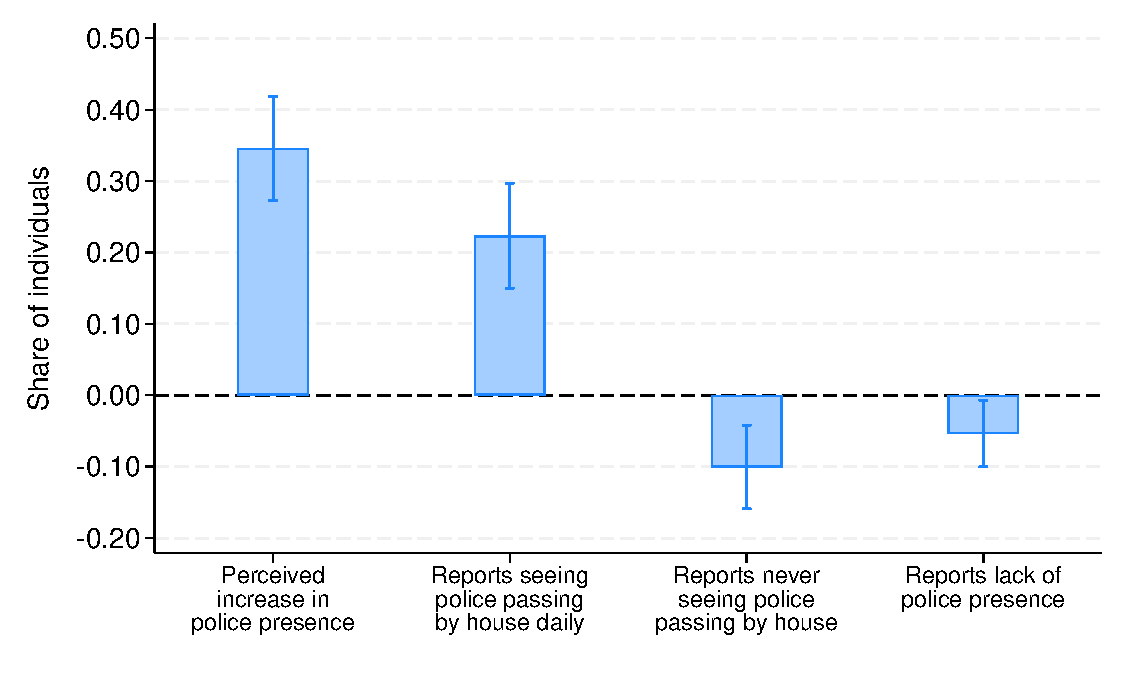
\includegraphics[width=\linewidth]{../manuscript/Graphs/results_policepresence.pdf}
        \caption{Effect on police presence}
    \end{subfigure}\hfill
    \begin{subfigure}[t]{0.44\textwidth}
        \centering
        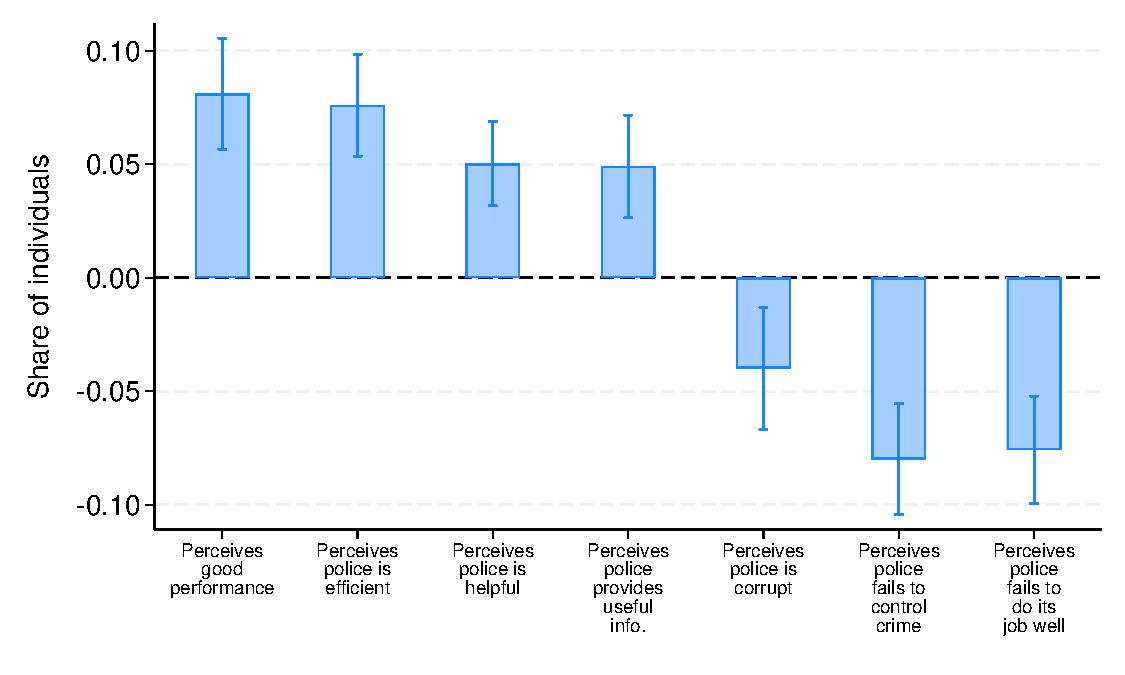
\includegraphics[width=\linewidth]{../manuscript/Graphs/combined_PCttest_2.pdf}
        \caption{Effect on perceived police performance}
    \end{subfigure}
    \\[6pt]
    \begin{subfigure}[t]{0.44\textwidth}
        \centering
        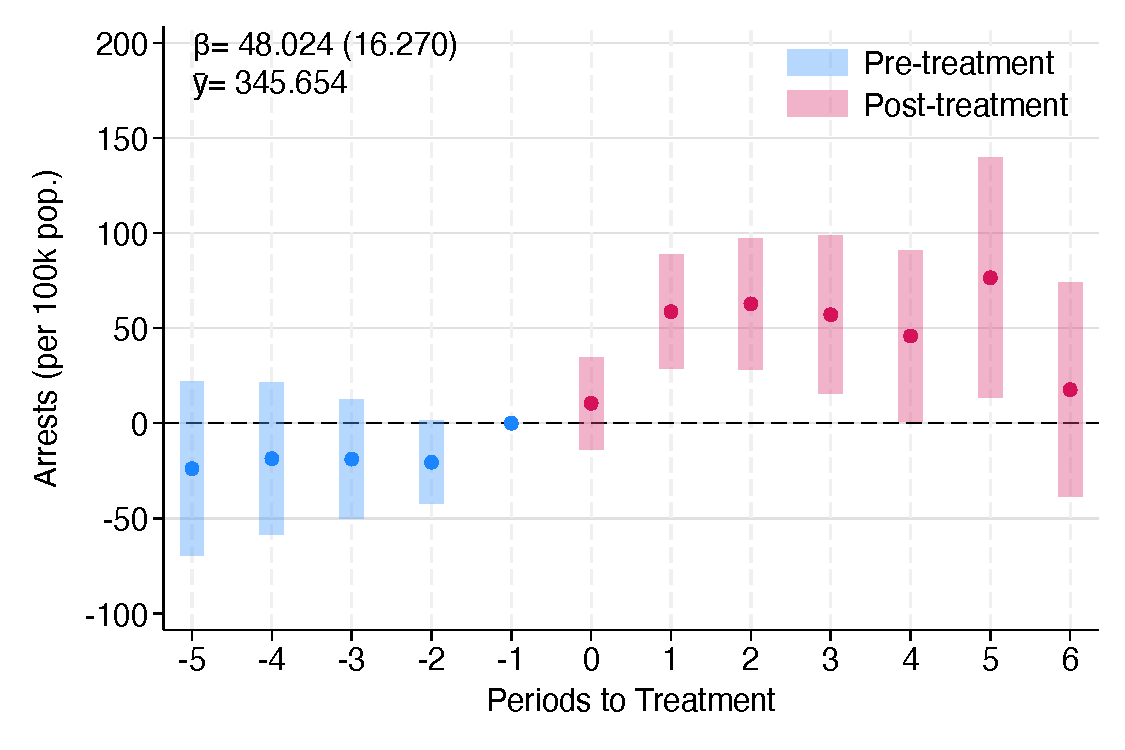
\includegraphics[width=\linewidth]{../manuscript/Graphs/totalarrestscrime_allcomunas.pdf}
        \caption{Arrests (per 100k pop.)}
    \end{subfigure}\hfill
    \begin{subfigure}[t]{0.44\textwidth}
        \centering
        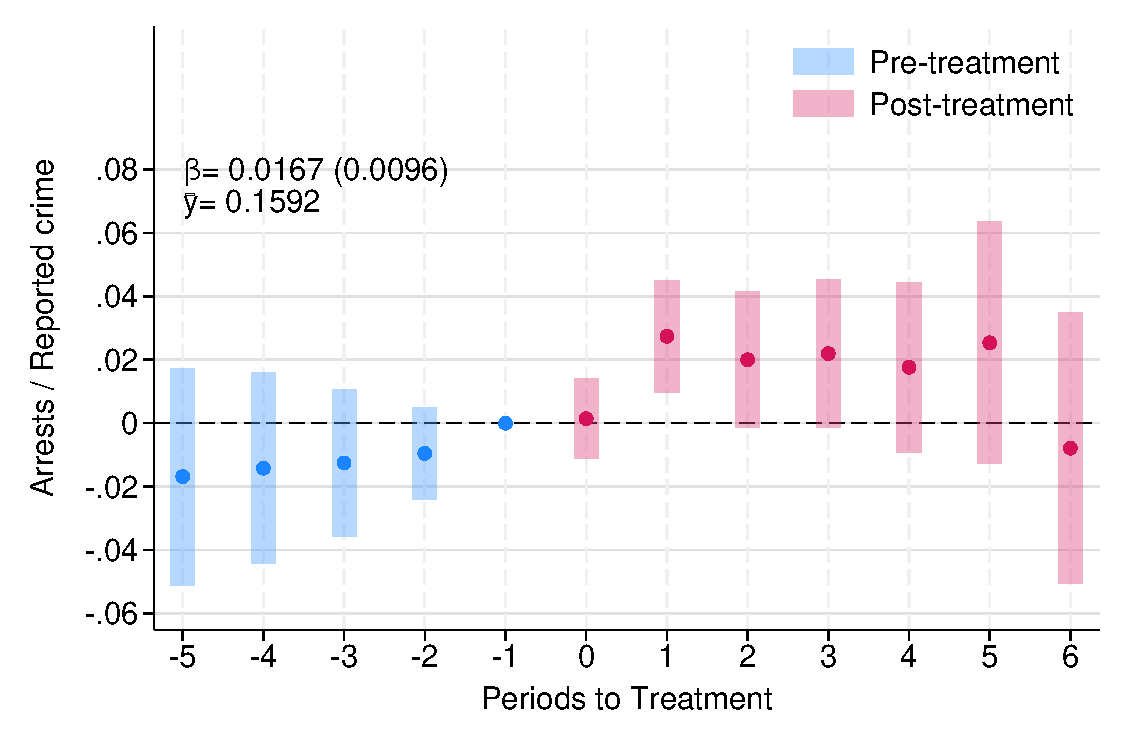
\includegraphics[width=\linewidth]{../manuscript/Graphs/arrests_over_reportedcrime_allcomunas.pdf}
        \caption{Arrests / Reported crime}
    \end{subfigure}
    \\[6pt]
    \begin{subfigure}[t]{0.44\textwidth}
        \centering
        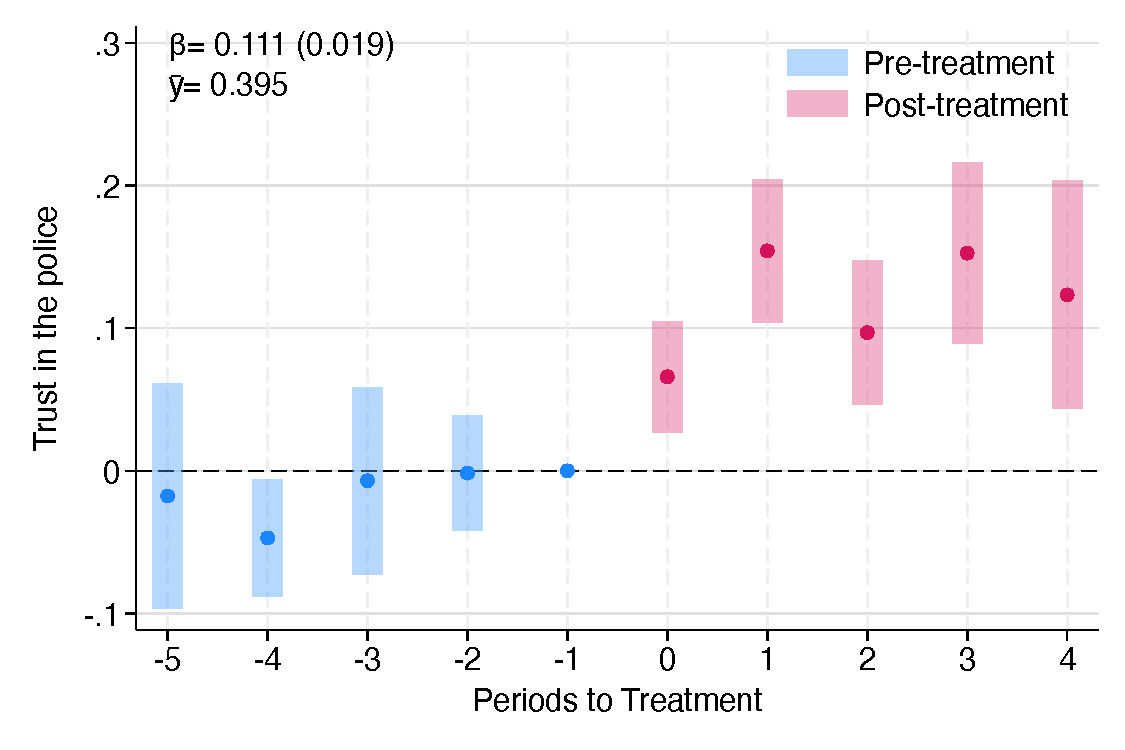
\includegraphics[width=\linewidth]{../manuscript/Graphs/results_trustcarabineros.pdf}
        \caption{Trust in the police}
    \end{subfigure}
    \\[8pt]
    \begin{minipage}{0.99\textwidth}
    \footnotesize Notes: Panel (a) reports the effects on perceived police presence. Panel (b) reports perceived police performance in 2005, comparing municipalities where \emph{Plan Cuadrante} was already implemented before 2006 with municipalities where it was implemented after 2005. Panels (c), (d), and (e) report dynamic event-study estimates for arrests per 100,000 inhabitants, the ratio of arrests to reported crime, and trust in the police. The estimation follows \citet{Callaway}. The graphs display estimated coefficients and 95\% confidence intervals. Standard errors are clustered at the municipality level using the wild bootstrapping procedure.
    \end{minipage}
\end{figure}
}

\clearpage

{\renewcommand{\thefigure}{B.6}
\begin{figure}[H]
    \centering
    \caption{Timing of Adoption of \emph{Plan Cuadrante} and Perceived Police Performance}
    \label{fig:balance_doseresponse}
    \begin{subfigure}{0.495\textwidth}
        \centering
        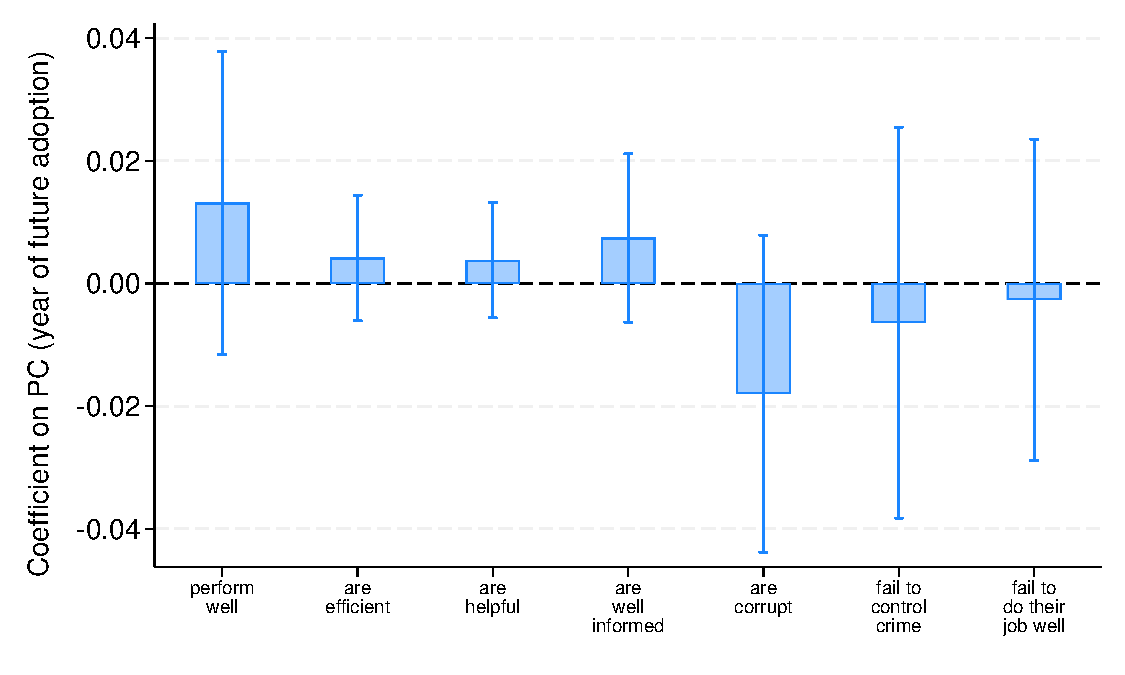
\includegraphics[width=\textwidth]{../manuscript/Graphs/balance_carabperc.pdf}
        \caption{Year of adoption and police performance before adoption}
    \end{subfigure}%
    ~
    \begin{subfigure}{0.495\textwidth}
        \centering
        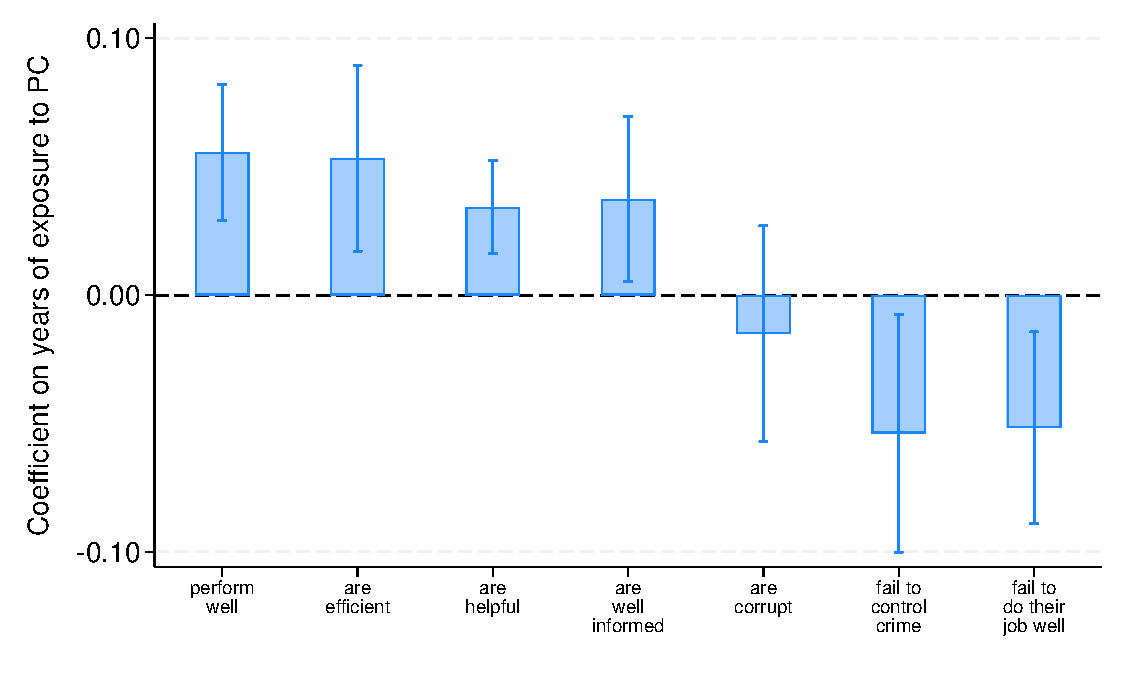
\includegraphics[width=\textwidth]{../manuscript/Graphs/doseresponse_carabperc.pdf}
        \caption{Years exposed to \emph{Plan Cuadrante} (dose response)}
    \end{subfigure}%
    \\[12pt]
    \begin{minipage}{0.99\textwidth}
    Notes: The figure considers seven measures of police performance: the share of respondents who perceive police performance as good, and who perceive the police to be efficient, helpful, well informed, corrupt, failing to control crime, and failing to do their job well. Using the sample of municipalities that adopted \emph{Plan Cuadrante} after 2005, panel (a) examines whether the future timing of adoption of \emph{Plan Cuadrante} is correlated with perceived police performance in 2005, before the introduction of the program. Panel (b) reestimates the same comparison as Figure \ref{fig:figure05}, replacing the binary adoption indicator with the municipality's number of years of exposure to \emph{Plan Cuadrante} as of 2005. In both panels, each bar plots the coefficient from a separate regression of one performance measure. The graphs display the estimated coefficients and 95\% confidence intervals.
    \end{minipage}
\end{figure}
}

\clearpage

